%%%%%%%%%%%%%%%%%%%%%%%%%
% !TeX spellcheck = pl_PL
\documentclass{beamer}
\usepackage[utf8]{inputenc}                                      
\usepackage[T1]{fontenc}                            
\usepackage[polish]{babel}                           
\selectlanguage{polish}
\usepackage{indentfirst} 
%\usepackage{tabularx}
%\usepackage{color}
%\usepackage{hyperref} 
%\usepackage{fancyhdr}
%\usepackage{listings}
%\usepackage{stmaryrd}
\usepackage{graphicx}
\usepackage{amssymb,amsmath}  % use mathematical symbols
\usepackage{pifont}
\usepackage{booktabs}
\usepackage{wasysym}
\usepackage[caption=false]{subfig}
 

%\usetheme{Luebeck}
%\usetheme{Berkeley}
%\usecolortheme{albatross}
%\usetheme{PaloAlto}
%\usetheme{Warsaw}
\usecolortheme{crane}
%\usecolortheme{albatross}
%\useoutertheme{infolines}
\useoutertheme{miniframes}

 
 


\newcommand{\zaleta}{\ding{52}}
\newcommand{\wada}{\ding{54}}

%\AtBeginSection[]
%{
% \begin{frame}
%  \frametitle{Plan}
%  \small
%  \tableofcontents[currentsection, hideallsubsections]
%  \normalsize
% \end{frame}
%}
%
%\newcommand{\plan}{% outline 
%\AtBeginSection[]
%{
% \begin{frame}
%  \frametitle{Gdzie jesteśmy?}
%  \small
%  \tableofcontents[currentsection, hideallsubsections]
%  \normalsize
% \end{frame}
%}
%}


\newcommand{\planCaly}{% outline 
\AtBeginSection[]
{
 \begin{frame}
  \frametitle{Plan}
  \small
  \tableofcontents[hideallsubsections]
  \normalsize
 \end{frame}
}
}





% numery stron
\setbeamertemplate{footline}[frame number]

\begin{document}
%\plan
% strona tytulowa
\title[]% short title
{Narzędzie do wizualizacji działań w sieciach przepływowych} % full title
%\subtitle {}
\author[ ]{Mateusz Forczmański\\promotor: dr inż. Agnieszka Debudaj-Grabysz}
\institute[PolSl]{Politechnika Śląska}

\ifpdf
\logo{\includegraphics[width=0.1\textwidth]
{img/polsl-white.pdf}}
\fi

\date{\today}


% this is used in the pdf information
\subject{Narzędzie do wizualizacji działań w sieciach przepływowych}

\begin{frame}%[plain]
        \titlepage
\end{frame}

\begin{frame}
	\frametitle{Plan}
   \tableofcontents[hideallsubsections]
\end{frame}

\section{Wprowadzenie}
\begin{frame}[<+(1)->]\frametitle{Cele pracy inżynierskiej}
	\begin{itemize}
		\item Aplikacja edukacyjna
		\item Wprowadzanie własnych sieci
		\item Kontrola poprawności
		\item Zobrazowanie algorytmów
		\item Śledzenie procesu krok po kroku
		\item Serializacja sieci
	\end{itemize}	
\end{frame}
\begin{frame}\frametitle{Podstawowe pojęcia}
	\begin{center}
		\includegraphics[width=0.9\textwidth]{./img/siec05}
	\end{center}
\begin{itemize}
\item Sieć przepływowa $ \rightarrow $ układ rur i połączeń
\item Wierzchołek $ \rightarrow $ punkt przerzutowy
\item Łuk $ \rightarrow $ przepustowość i przepływ
\item Źródło $ s $
\item Ujście $ t $
\end{itemize}	
\end{frame}

\section{Maksymalny przepływ}
\begin{frame}\frametitle{Wyznaczanie maksymalnego przepływu}
	\begin{center}
		\includegraphics<1>[width=0.9\textwidth]{./img/siec01}
		\includegraphics<2>[width=0.9\textwidth]{./img/siec02}
		\includegraphics<3>[width=0.9\textwidth]{./img/siec03}
		\includegraphics<4>[width=0.9\textwidth]{./img/siec04}
	\end{center}
\end{frame}
\section{Sieci przepływowe}
\subsection{Właściwości sieci przepływowej}
\begin{frame}\frametitle{Warunek przepustowości}
	\begin{center}
		\includegraphics[width=0.8\textwidth]{./img/warunek_1}
	\end{center}
\end{frame}
\begin{frame}\frametitle{Warunek skośnej symetryczności}
	\begin{center}
		\includegraphics[width=0.8\textheight]{./img/warunek_2}
	\end{center}
\end{frame}
\begin{frame}\frametitle{Warunek zachowania przepływu}
	\begin{center}
		\includegraphics[width=0.8\textwidth]{./img/warunek_3}
	\end{center}
\end{frame}

\section{Algorytmy}
\begin{frame}\frametitle{Sieć residualna}
	\begin{figure}
		\subfloat[Sieć pierwotna]{\includegraphics[width=0.45\textwidth]{./img/residual_pres2}}\quad
		\subfloat[Sieć residualna]{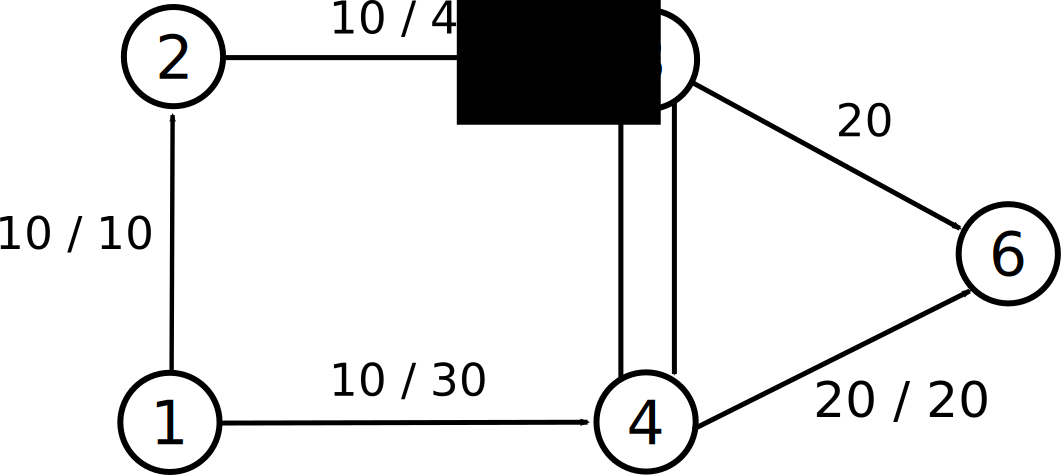
\includegraphics[width=0.45\textwidth]{./img/residual_pres1}}
		\caption{Tworzenie sieci residualnej}
	\end{figure}
\end{frame}
\begin{frame}\frametitle{Algorytm Forda-Fulkersona}
	\begin{center}
		\includegraphics[width=0.9\textwidth]{./img/pres_ff1_1}\\\par\bigskip
		\includegraphics[width=0.9\textwidth]{./img/pres_ff2_1}
	\end{center}
\end{frame}
\begin{frame}\frametitle{Algorytm Dinica}
	\begin{center}
		\includegraphics<1>[width=0.9\textwidth]{./img/pres_dinic1}\\\par\bigskip
		\includegraphics<1>[width=0.9\textwidth]{./img/pres_dinic2}
	\end{center}
\end{frame}
\begin{frame}\frametitle{Algorytm MKM}
	\begin{center}
		\includegraphics<1>[width=0.9\textwidth]{./img/pres_mkm1}\\\par\bigskip
		\includegraphics<1>[width=0.9\textwidth]{./img/pres_mkm2}
	\end{center}
\end{frame}

\section{Działająca aplikacja}
\subsection{Interfejs graficzny aplikacji}
\begin{frame}\frametitle{Okno główne}
	\begin{center}
		\includegraphics[width=0.9\textwidth]{./img/pres_screen1}
	\end{center}
\end{frame}
\begin{frame}\frametitle{Okno algorytmu Forda-Fulkersona}
	\begin{center}
		\includegraphics[width=0.9\textwidth]{./img/pres_screen2}
	\end{center}
\end{frame}
\begin{frame}\frametitle{Okno algorytmu Dinica}
	\begin{center}
		\includegraphics[width=0.9\textwidth]{./img/pres_screen3}
	\end{center}
\end{frame}
\section{}
\begin{frame}\frametitle{Koniec}
	\centering
	\LARGE{\textbf{Dziękuję za uwagę}}
\end{frame}
%%%%%%%%%%%%%%%%%%%%%%%%%%%%%%%%%%%%%%%%%%%%%%%%%%%%%%%%%%%%%%%%%%%%%%%%


\end{document}


